\documentclass[]{beamer}

% Default size A0
% \usepackage[scale=1.1, size=a0]{beamerposter} % use scale from 1.1 to 1.2

% Size A1
% \usepackage[scale=0.77, size=a1]{beamerposter} % use scales around 0.8

% Use custom size to set poster's width and height.
\usepackage[scale=1.2, size=custom, width=120, height=100]{beamerposter} % use scale from 1.1 to 1.2
\usetheme{vegaposter} 


\addbibresource{refs.bib}
\usepackage{lipsum}

\title{On the broccoli fractional structure}
\author{Alexander Rosenbaum, Noname Student}
\supervisor{Group Supervisor 1, Group Supervisor 2}
\researchgroup{Important questions of stochastic calculus}

\begin{document}
\nocite{*} % This is needed to make sure that all references are included in the bibliography

\begin{frame}[t]
    \begin{columns}[t] % The whole poster consists of three major columns, the second of which is split into two columns twice - the [t] option aligns each column's content to the top
     
    \begin{column}{\lrmargin}\end{column} % Empty spacer column
    
    \begin{column}{\onecolwid} % The first column
     
    %----------------------------------------------------------------------------------------
    %	INTRODUCTION
    %----------------------------------------------------------------------------------------
    
    \begin{block}{Introduction}
    
    The fractional structure of broccoli refers to the different components or parts that make up a broccoli plant. Broccoli is a type of vegetable belonging to the cabbage family (\textit{Brassicaceae}) and is known for its dense clusters of green flower buds and stalks. 
    
    \end{block}
    
    %----------------------------------------------------------------------------------------
    %	OBJECTIVES
    %----------------------------------------------------------------------------------------
    
    \begin{alertblock}{Objectives}
    
    Here are the main parts of a broccoli plant:
    \begin{itemize}
        \item Floret: The florets are the small, tightly packed clusters that make up the head of broccoli. These are the edible portions of the plant and are composed of immature flower buds.

    	\item  Stalk: The stalk of broccoli is the main central stem that supports the florets. It is typically thick and sturdy, providing structural support for the head.

    	\item Leaves: Broccoli plants have large, dark green leaves that extend from the stalk. While the leaves are not commonly consumed, they are edible and can be cooked or used in recipes, similar to other leafy greens.

    	\item Stem: The stem refers to the entire length of the main central stalk, including both the lower, thicker part (which supports the head) and the upper, thinner part that extends beyond the florets.

    	\item Roots: Although not typically visible or consumed as part of the broccoli we eat, broccoli plants have a root system that anchors them into the soil and absorbs nutrients and water.
    \end{itemize}
    
    \end{alertblock}
    
    %------------------------------------------------
    \begin{block}{Problem statement}
    These components together form the fractional structure of broccoli, with the florets being the most recognizable and commonly consumed part.
    \end{block}
    
    %----------------------------------------------------------------------------------------
    
    \end{column} % End of the first column
    
    \begin{column}{\sepwid}\end{column} % Empty spacer column
    
    \begin{column}{\twocolwid} % Begin a column which is two columns wide (column 2)
    
    \begin{columns}[t,totalwidth=\twocolwid] % Split up the two columns wide column
    
    \begin{column}{\onecolwid}\vspace{-.6in} % The first column within column 2 (column 2.1)
    
    %----------------------------------------------------------------------------------------
    %	MATERIALS
    %----------------------------------------------------------------------------------------
    
    \begin{block}{Materials}
    
     Broccoli exhibits fractal-like properties in its structure. A fractal is a mathematical concept that describes a pattern that repeats itself on different scales or magnifications. In the case of broccoli, the self-repeating pattern can be observed at different levels of its structure.
     
     If you examine a broccoli head closely, you will notice that it is composed of smaller, tightly packed clusters called florets. Each floret, in turn, is made up of even smaller clusters, and this pattern continues recursively. As you zoom in, you will find that the smaller clusters resemble the larger cluster they are part of.
    
    \end{block}
    
    %----------------------------------------------------------------------------------------
    
    \end{column} % End of column 2.1
        
    \begin{column}{\onecolwid}\vspace{-.6in} % The second column within column 2 (column 2.2)
    
    %----------------------------------------------------------------------------------------
    %	METHODS
    %----------------------------------------------------------------------------------------
    
    \begin{block}{Methods}
    
    In the case of broccoli, the main stalk branches out into smaller stalks, which then further divide into even smaller stalks, and so on. Each level of branching follows a similar pattern to the previous level, creating a self-repeating structure.

If you observe the florets of broccoli, you'll notice that they are also arranged in a fractal-like pattern. The florets are clustered together in a manner that resembles a miniature version of the overall shape of the broccoli head. As you zoom in, you'll find that each floret consists of even smaller florets, and this pattern continues.

    
    \end{block}
    
    %----------------------------------------------------------------------------------------
    
    \end{column} % End of column 2.2
    
    \end{columns} % End of the split of column 2 - any content after this will now take up 2 columns width
    
    %----------------------------------------------------------------------------------------
    %	IMPORTANT RESULT
    %----------------------------------------------------------------------------------------
    
    \begin{alertblock}{Broccoli is rough!}
    
     When we examine the structure of broccoli, we can observe repeated patterns that resemble the whole plant. The branching pattern of the main stem is reflected in the smaller branches, and these branches further divide into even smaller branches, creating a self-similar pattern.
    
    \end{alertblock} 
    
    %----------------------------------------------------------------------------------------
    
    \begin{columns}[t,totalwidth=\twocolwid] % Split up the two columns wide column again
    
    \begin{column}{\onecolwid} % The first column within column 2 (column 2.1)
    
    %----------------------------------------------------------------------------------------
    %	MATHEMATICAL SECTION
    %----------------------------------------------------------------------------------------
    
    \begin{block}{Mathematical Section}
    
    This self-similar pattern is characteristic of fractals. Fractals exhibit a property known as self-similarity, where parts of the object resemble the whole, or sections of the object resemble each other. 
    
    $$
    N = \varepsilon^{-D}
    $$
    
    The fractal nature of broccoli's structure is visually intriguing and has been studied by scientists and mathematicians interested in the beauty and mathematical properties of natural forms. 
    
    The branching pattern of a broccoli plant follows a fractal geometry known as a self-similar fractal. A self-similar fractal is one in which smaller parts resemble the overall shape or structure of the whole.  
    \end{block}
   
    
    %----------------------------------------------------------------------------------------
    
    \end{column} % End of column 2.1
    
    \begin{column}{\onecolwid} % The second column within column 2 (column 2.2)
    
    %----------------------------------------------------------------------------------------
    %	RESULTS
    %----------------------------------------------------------------------------------------
    
    \begin{block}{Results}
    
    \begin{figure}
    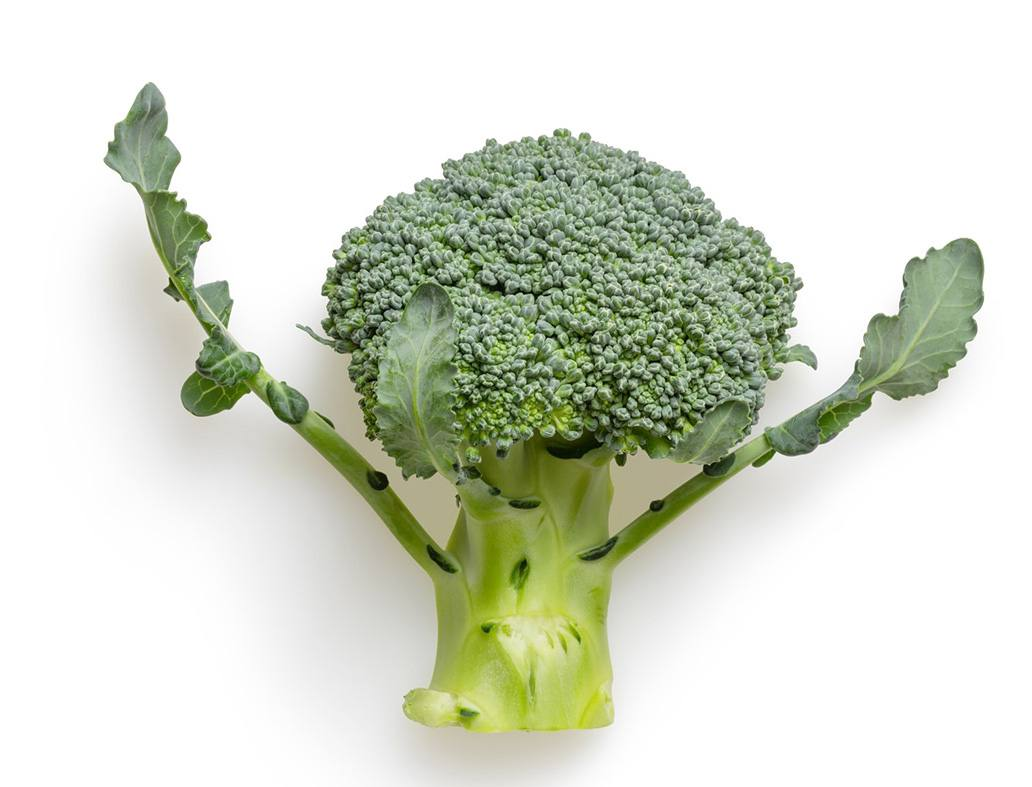
\includegraphics[width=0.8\linewidth]{figures/placeholder.jpg}
    \caption{Figure caption}
    \end{figure}
    
    Nunc tempus venenatis facilisis. Curabitur suscipit consequat eros non porttitor:
    
    \begin{table}
    \vspace{2ex}
    \begin{tabular}{l l l}
    \hline
    \textbf{Measurements} & \textbf{Dimension estimator $\hat D$} \\
    \hline
    Try 1 & 2.66 \\
    \hline
    \end{tabular}
    \caption{Empirical analysis of the Hausdorff dimension}
    \end{table}
    
    \end{block}
    
    %----------------------------------------------------------------------------------------
    
    \end{column} % End of column 2.2
    
    \end{columns} % End of the split of column 2
    
    \end{column} % End of the second column
    
    \begin{column}{\sepwid}\end{column} % Empty spacer column
    
    \begin{column}{\onecolwid} % The third column
    
    %----------------------------------------------------------------------------------------
    %	CONCLUSION
    %----------------------------------------------------------------------------------------
    
    \begin{block}{Conclusion}
    This recursive branching and self-similar pattern in the structure of broccoli are what make it an example of a fractal in nature. Fractals can be found in various natural phenomena, and broccoli serves as a visually appealing example of fractal geometry in plants.

    In conclusion, broccoli exhibits fractal characteristics in its structure. The self-repeating patterns and recursive branching observed in broccoli's stalks and florets resemble the mathematical concept of fractals. This self-similarity at different scales is a defining characteristic of fractals. Therefore, broccoli can be considered an example of a fractal in nature.
    
    The branching pattern of the broccoli plant, as well as the arrangement of its florets, follows a self-similar fractal geometry. This means that the smaller parts of broccoli, such as the stalks and florets, resemble the overall shape and structure of the whole plant. The fractal nature of broccoli's structure adds to its visual appeal and highlights the presence of mathematical patterns in nature.
    
    Follow us in \href{https://t.me/vega_institute}{Telegram}.
    
    \end{block}
    
    %----------------------------------------------------------------------------------------
    %	REFERENCES
    %----------------------------------------------------------------------------------------
    
    \begin{block}{References}
    
%    \nocite{*} % Insert publications even if they are not cited in the poster
    \printbibliography \vspace{0.75in}
    
    \end{block}
    
    \end{column} % End of the third column
    
    \begin{column}{\lrmargin}\end{column} % Empty spacer column
    
    \end{columns} % End of all the columns in the poster
    \end{frame} % End of the enclosing frame
\end{document}